\pdfoptionpdfminorversion=5
\documentclass{beamer}

\mode<presentation>
{
  \usetheme{Malmoe}
}

\usepackage{listings}
\usepackage[english]{babel}
\usepackage[latin1]{inputenc}
\usepackage{times}
\usepackage[T1]{fontenc}
\usepackage{eurosym}

\title[CF3 demo]{Coolfluid 3: Demonstration of current capabilities}

\date{16 Nov 2011}

\begin{document}

\section{Introduction}


\frame{ \frametitle{Coolfluid 3}
\begin{itemize}
 \item Started based on CF2 experience, as natural evolution
 \item Focus on flexibility and inter-operability between solvers
 \item Inter-institutional project
 \begin{itemize}
  \item IDIHOM
  \item PhD projects
  \item Institutions involved: VKI, VUB, RMA
 \end{itemize}
\end{itemize}
}

\frame{ \frametitle{People}
In alphabetical order:
\begin{itemize}
  \item B\'{a}nyai, Tam\'{a}s (VKI-AR):
  \item Deconinck, Willem (VUB):
  \item Gasper, Quentin (VKI-CC):
  \item Janssens, Bart (RMA,VKI???):
  \item Quintino, Tiago (freelance):
  \item Scholl, Sebastian (VKI-TU):
  \item Vymazal, Martin (VKI-AR):
\end{itemize}
}


\frame{ \frametitle{Development model}
\begin{columns}
\begin{column}{6cm}
\begin{itemize}
 \item Open-source, GNU v3
 \item Stored on GitHub
 \begin{itemize}
  \item Version control: git
  \item Everyone can join
  \item Already 18 watchers
  \item Ensures growth potential
 \end{itemize}
 \item CMake as build system
 \begin{itemize}
  \item Platform independence
 \end{itemize}
 \item CTest
 \begin{itemize}
  \item UTest, ATest, PTest
  \item Continuous \& nightly builds
  \item Dashboard
  \item Code coverage
 \end{itemize}

\end{itemize}
\end{column}
\begin{column}{4cm}
\begin{center}
 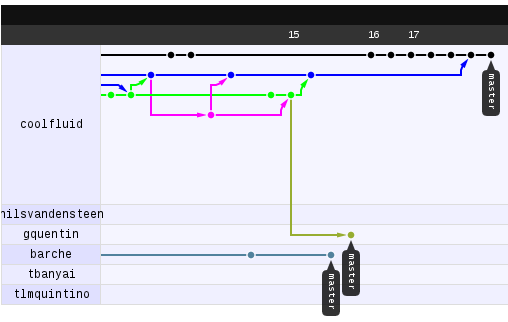
\includegraphics[width=4cm]{figs/github}\\
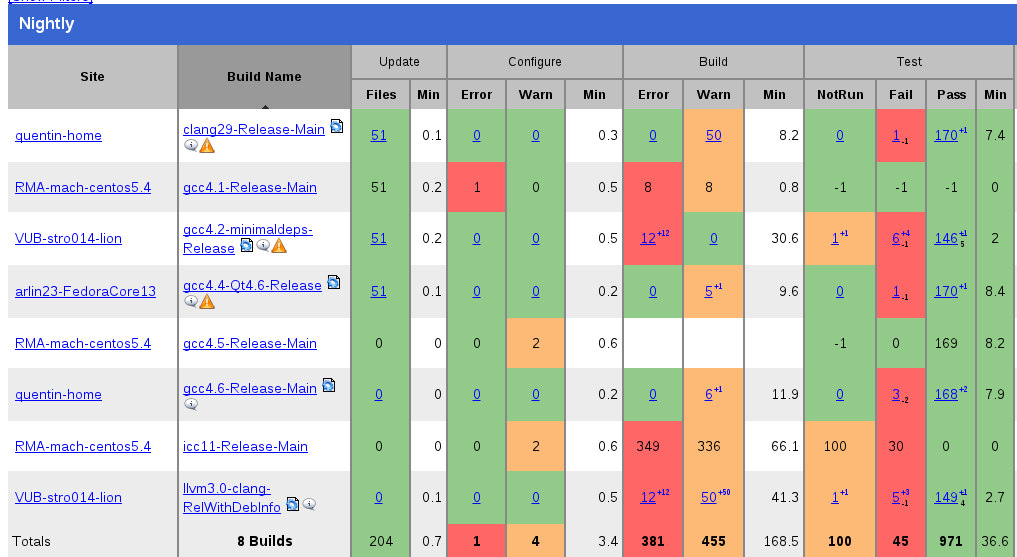
\includegraphics[width=4cm]{figs/dash}
\end{center}
\end{column}
\end{columns}
}


\section{Component System}

\begin{frame}
 \frametitle{Component System}
\begin{itemize}
 \item Structure
 \begin{itemize}
  \item Tree of components, parents own children
  \item Access through ``file system'' path interface
 \end{itemize}
 \item Dynamic API
 \begin{itemize}
  \item Configuration using options
  \item Function calls through ``signals''
  \item Network-transparent
  \item Used for automatic UI and script binding interface
 \end{itemize}
 \item C++ API in the ``common'' library
\end{itemize}
\end{frame}


\section{Framework}
%\section{GUI}

\frame{\frametitle{Framework}
\begin{itemize}
 \item GUI
 \item Mesh
 \item Fields
 \item Python
 \item Linear System Solver Interface
 \item Parallelization
\end{itemize}
}

\frame{\frametitle{Python}
Component system and signals are make it ideal to prepare blocks of codes, like LEGO, and the final order of execution is assembled in a python script.
\begin{itemize}
 \item CF3 code parts are inidividually executed upon python calls
 \item Therefore CF3 is one big box of LEGO
 \item Python built-in things can be used
 \item Console in GUI currently developed by ESI student joining GUI and Python advantages
\end{itemize}
}



\begin{frame}
 \frametitle{GUI}
 \begin{itemize}
  \item Client-server system
  \item Server can control a parallel simulation on a cluster
  \item Mesh visualization using Paraview
  \item Dynamic generation, plugin authors don't need to do GUI programming
 \end{itemize}
\end{frame}

%\section{Mesh}

\begin{frame}
  \frametitle{Mesh}
    Features:
    \begin{itemize}
      \item Flexible functional data structure built on component environment
      \item Unlimited number of meshes
      \item Unlimited nesting of regions to allow CAD-like topologies
      \item Unstructured meshes for complex geometries
      \item Support for both Continuous / Discontinuous fields
      \item Support for fields based on arbitrary shape-function
      \item Parallel distributed and loadbalanced
    \end{itemize}
\end{frame}

\frame[containsverbatim]{ \frametitle{CAD-like topology:\; mesh.print\_tree() }
\begin{verbatim}
  Mesh                              Mesh
    + Topology                      Region
        - Flow                      Region
        + AirPlane                  Region
            + Wings                 Region
            |   + LeftWing          Region
            |   |   - Patch1        Region
            |   |   - Patch2        Region
            |   - RightWing         Region
            + Fuselage              Region
                + Quads             Elements
                + Triags            Elements
\end{verbatim}
  % \begin{itemize}
  %   \item Elements are grouped per type inside these regions
  %   \begin{itemize}
  %     \item Memory optimized per element type (connectivity tables)
  %     \item Optimized numerical algorithms per element type possible.
  %   \end{itemize}
  % \end{itemize}
}

\frame{ \frametitle{Spaces and Fields}
  \begin{block}{Spaces}
    \begin{itemize}
      \item Parallel representation of the mesh, or part of the mesh
      \item Defined by shape-function and connectivity table
      \item Continuous/Discontinuous
      \item Accurate interpolation between spaces
    \end{itemize}
  \end{block}
\begin{block}{Fields}
  \begin{itemize}
    \item Defined in 1 space (Not necessarily the entire mesh)
    \item Continuous/Discontinuous (e.g. cell-centred finite volume)
    \item Synchronizable using MPI
    \item Coordinates are a field like any other
  \end{itemize}
\end{block}
}
\frame{ \frametitle{Spaces and Fields}

Include here graphical view of spaces

}


\frame[containsverbatim]{ \frametitle{Spaces and Fields}
\begin{columns}
\begin{column}{0.4 \textwidth}
\begin{verbatim}
Mesh
+ Topology
| - Flow
|   - Triangles
|   - Quads
+ GeometrySpace
| - Coordinates
| - WallDistance
+ SolutionSpace
  - Coordinates
  - Solution
  - Residual
\end{verbatim}
\end{column}
\begin{column}{0.6 \textwidth}
\begin{verbatim}
Quads
- ElementType
+ Spaces
  + GeometrySpace
  | - ShapeFunction (P1)
  | - ConnectivityTable
  + SolutionSpace
    - ShapeFunction (P3)
    - ConnectivityTable
\end{verbatim}
\end{column}
\end{columns}
}

\frame{ \frametitle{Mesh Manipulations}
\begin{block}{Create new regions and elements}
  \begin{itemize}
    \item Build faces
    \item Remove or merge regions
    \item Reorganize regions
  \end{itemize}
\end{block}
\begin{block}{Create new spaces and fields}
  \begin{itemize}
    \item High-order solution-space
    \item P-multigrid with multiple solution-spaces
    \item Simple to create and access.
  \end{itemize}
\end{block}
}

\frame{ \frametitle{Mesh IO}
Distributed: meshes can be larger than memory of 1 processor
Loadbalancing: Reduce communication between processors
\begin{block}{Generation}
  \begin{itemize}
    \item Line, Rectangle, Box
    \item Block-based assembly, with grading
  \end{itemize}
\end{block}
\begin{block}{Input}
  \begin{itemize}
    \item Gmsh, Neutral, CGNS, OpenFOAM dict
  \end{itemize}
\end{block}
\begin{block}{Output}
  \begin{itemize}
    \item Gmsh, Tecplot, VTK (Paraview), Neutral, CGNS
  \end{itemize}
\end{block}
}

%\section{Linear System Solver Interface}

\frame{ \frametitle{Linear System Solver Interface}
Interface: avoid being tailored to one specific LSS library.\\
Distributed: uses the parallel layer and mesh.\\
Currently works with: Trilinos (Sandia National Labs).\\
\begin{itemize}
  \item The best open source package (in my opinion)
  \item Very active research and development (Efficiency, GPU,...)
  \item Parallel via MPI
  \item Many type of solvers through a unified XML config file
  \begin{itemize}
    \item Direct solvers (Amesos KLU, Metis, ParMetis)
    \item BiCGStab and friends (Belos,Aztec)
    \item GMRES ILU, Block GMRES and friends (Belos, Aztec)
    \item Algebraic MultiGrid (ML)
    \item ...
  \end{itemize}
\end{itemize}
}

\frame{ \frametitle{Trilinos Configuration Example (GMRES+AMG)}
  <Parameter isUsed="true" name="Linear Solver Type" type="string" value="Belos"/>
  <ParameterList name="Linear Solver Types">
    <ParameterList name="Belos">
      <Parameter isDefault="true" isUsed="true" name="Solver Type" type="string" value="Block GMRES"/>
      <ParameterList name="Solver Types">
        <ParameterList name="Block GMRES">
          <Parameter name="Verbosity" type="int" value="4"/>
          <Parameter name="Output Frequency" type="int" value="-1"/>
          <Parameter name="Adaptive Block Size" type="bool" value="true"/>
          <Parameter name="Block Size" type="int" value="1"/>
          <Parameter name="Convergence Tolerance" type="double" value="1e-3"/>
          <Parameter name="Explicit Residual Scaling" type="string" value="Norm of Initial Residual"/>
          <Parameter name="Explicit Residual Test" type="bool" value="false"/>
          <Parameter name="Flexible Gmres" type="bool" value="true"/>
          <Parameter name="Implicit Residual Scaling" type="string" value="Norm of Preconditioned Initial Residual"/>
          <Parameter name="Maximum Iterations" type="int" value="50"/>
          <Parameter name="Maximum Restarts" type="int" value="20"/>
          <Parameter name="Num Blocks" type="int" value="20"/>
          <Parameter name="Orthogonalization" type="string" value="IMGS"/>
          <Parameter name="Orthogonalization Constant" type="double" value="-1"/>
          <Parameter name="Show Maximum Residual Norm Only" type="bool" value="false"/>
          <Parameter name="Timer Label" type="string" value="Belos"/>
        </ParameterList>
      </ParameterList>
    </ParameterList>
  </ParameterList>
}

\frame{ \frametitle{Trilinos Configuration Example (GMRES+AMG)}
  <Parameter name="Preconditioner Type" type="string" value="Ifpack"/>
  <ParameterList name="Preconditioner Types">
    <ParameterList name="ML">
      <Parameter name="Base Method Defaults" type="string" value="SA"/>
      <ParameterList name="ML Settings">
        <Parameter name="aggregation: damping factor" type="double" value="1.333"/>
        <Parameter name="aggregation: type" type="string" value="Uncoupled-MIS"/>
        <Parameter name="coarse: max size" type="int" value="1024"/>
        <Parameter name="coarse: pre or post" type="string" value="post"/>
        <Parameter name="coarse: sweeps" type="int" value="2"/>
        <Parameter name="coarse: type" type="string" value="Amesos-KLU"/>
        <Parameter name="default values" type="string" value="NSSA"/>
        <Parameter name="eigen-analysis: iterations" type="int" value="10"/>
        <Parameter name="eigen-analysis: type" type="string" value="cg"/>
        <Parameter name="increasing or decreasing" type="string" value="increasing"/>
        <Parameter name="max levels" type="int" value="25"/>
        <Parameter name="prec type" type="string" value="MGW"/>
        <Parameter name="smoother: damping factor" type="double" value="1"/>
        <Parameter name="smoother: pre or post" type="string" value="post"/>
        <Parameter name="smoother: sweeps" type="int" value="2"/>
        <Parameter name="smoother: type" type="string" value="symmetric Gauss-Seidel"/>
      </ParameterList>
    </ParameterList>
  </ParameterList>
}

\section{Solvers}

\frame{\frametitle{Spectral Finite Difference}
SDM
}

\frame{\frametitle{Unstructured Finite Element}
UFEM
}

\frame{\frametitle{Residual Distribution}
RDM
}

\section{Conclusion}

\begin{frame}
 \frametitle{Current abilities}
\begin{itemize}
 \item Python scripting: 
  \begin{itemize}
   \item parametrization
   \item optimalization
   \item error analysis
  \end{itemize}
 \item Spectral difference
 \item Incompressible Finite Element solver
 \item Residual Distribution
 \item Proto language
 \item Parallelization
 \item LSS interface
\end{itemize}
\end{frame}


\end{document}
